\documentclass[12pt, a4paper]{article}

\usepackage[utf8]{inputenc}
\usepackage[T1]{fontenc}
\usepackage{amsmath, amssymb}
\usepackage{booktabs}
\usepackage{graphicx}
\usepackage{hyperref}
\usepackage{natbib}
\usepackage{geometry}
\usepackage{setspace}
\usepackage{float}
\usepackage{tabularx}

\geometry{margin=1in}
\onehalfspacing

\title{Replicating Ertan, Page, and Putterman (2009) at Original Parameters with Persistent-Memory LLM Agents}

\author{%
  Tuna G\"ul\\
  Bo\u{g}azi\c{c}i University
  \and
  Claude\\
  Anthropic
}

\date{\today}

\begin{document}

\maketitle

\begin{abstract}
We re-replicate the public goods voting experiment of \citet{ertan2009who} using Large Language Model (LLM) agents connected to a real \texttt{oTree} server, under two changes relative to our prior replication. First, we match the original paper's experimental parameters exactly---groups of four, an endowment of ten tokens, and a punishment cost ratio of $1{:}4$---rather than the scaled-up parameters used previously. Second, we give each agent persistent chat memory across all pages of the experiment, so that earlier decisions and instructions remain visible when the agent reasons about later ones. We compare two conditions at $N=50$ each: default agents with no personality assignment, and agents assigned random Big Five personalities drawn from US adult norms. With a sufficiently large reasoning-token budget (\texttt{max\_tokens}$=128{,}000$), both conditions complete $50/50$ agents and $0$ field failures, eliminating the dropout pathology we previously diagnosed as reasoning-token exhaustion on the cooperative condition. The two conditions differ sharply. Default agents contribute almost nothing at baseline ($M=0.76$), respond rationally to the punish-high-only regime by contributing exactly zero, and vote against allowing punishment of low contributors at a rate of $56\%$. Personality agents contribute more at baseline ($M=5.30$, $d=-2.25$), contribute positively even when cooperation is penalised ($M=2.42$ under punish-high-only), and vote $90\%$ in favor of allowing punishment of low contributors. Both conditions vote $0\%$ for punishment of high contributors, matching the original paper's headline institutional finding. Within each condition, a Friedman test confirms that the four punishment regimes produce significantly different contributions from the same agent ($p<0.001$). We present the full statistical chain---Mann--Whitney with Bonferroni correction, chi-square for voting, Friedman for within-subject regime effects, and Cohen's $d$ for effect sizes---and discuss what changes and what does not relative to our prior scaled-parameter replication.

\medskip
\noindent\textbf{Keywords:} LLM agents, behavioral economics, public goods game, Big Five personality, BFI-2, oTree, replication, persistent memory, Homo Silicus
\end{abstract}

%----------------------------------------------------------------------
\section{Introduction}
%----------------------------------------------------------------------

The appeal of LLM-based behavioral economics is concrete: a replication that would cost thousands of dollars and weeks of recruitment with human subjects can be run for under a dollar and an afternoon with LLM agents. The tradeoff is equally concrete: LLM agents are not humans, and whether their behavior approximates human behavior with enough fidelity to be useful is an empirical question that has to be answered one paradigm at a time.

Our prior replication \citep{gul2026who} of \citet{ertan2009who} established a first-order positive answer for the institutional-choice part of that paper: default LLM agents, with no personality prompt, reproduce the paper's qualitative voting pattern (near-universal support for punishing low contributors, zero support for punishing high contributors) in a single shot, without the thirty periods of play humans needed to converge on that institution. That replication also surfaced two findings worth revisiting. First, we had scaled the experimental parameters up from the original (groups of five instead of four, an endowment of twenty instead of ten, a punishment cost ratio of $1{:}3$ instead of $1{:}4$), which left an uncomfortable footnote between our numbers and the original paper's numbers. Second, a hyper-cooperative condition we ran had a severe form-completion failure ($7/50$ on the punishment page), which we traced to reasoning-token exhaustion in the model we used (\texttt{step-3.5-flash}, with a $16{,}000$-token budget).

This paper re-runs the experiment under two changes designed to address both issues.

First, \textbf{exact parameter matching}. We use the original paper's groups of four, endowment of ten, and punishment cost ratio of $1{:}4$. Absolute contribution numbers are now directly comparable to the original paper on the same unit scale, rather than being translatable only through a scaling argument. We also rescaled the punishment-page group profiles accordingly, so that the three hypothetical groups still capture the ``all cooperate / mixed / one free-rider'' distinctions the original paper made but on a three-other-members, ten-token-endowment basis.

Second, \textbf{persistent-memory chat mode}. In our prior replication, each page was answered by an independent LLM call with fresh context. We now maintain a single conversation across every page of the experiment, including between-page info screens. The agent sees its own previous decisions, the running game state, and any interstitial text when reasoning about the next decision. This changes an LLM agent from a series of disconnected stateless responses into a persistent participant more closely analogous to a human playing through an experimental session end to end. We report results under this chat mode only, noting along the way how the shape of the answers differs from the stateless mode when we've been able to compare directly.

Third, as a measurement issue rather than a design change, we increased the reasoning-token budget from $16{,}000$ to $128{,}000$. The previous budget was comfortable for the default condition but tight for personality-prompted agents on reasoning-heavy questions, and it was the mechanism behind our prior hyper-cooperative dropout. With the new budget, both of the conditions reported here complete $50/50$ agents with zero field failures, and we don't have to carve out a special descriptive-only paragraph for a half-dropped condition.

Our contributions are:
\begin{enumerate}
  \item A parameter-faithful replication of \citet{ertan2009who} with $N=50$ default and $N=50$ random-personality agents, using the exact same group size, endowment, and punishment cost ratio as the original.
  \item Confirmation that the voting result from our prior paper carries through under the new parameters and chat-mode memory: $0\%$ of agents vote for punishment of high contributors in either condition, matching the original paper's institutional-choice result exactly.
  \item A full statistical chain applied to the replication: Mann--Whitney $U$ with Bonferroni correction, chi-square for voting, Friedman tests for within-subject regime effects, and Cohen's $d$ for effect sizes, instead of the pairwise-Mann--Whitney-only chain in our prior paper.
  \item Confirmation that our prior hyper-cooperative dropout was a \texttt{max\_tokens} artifact rather than a behavioral refusal: at $128{,}000$ tokens there is no dropout in either condition, consistent with the reasoning-budget-exhaustion diagnosis we gave at the time.
\end{enumerate}

%----------------------------------------------------------------------
\section{Related Work}
%----------------------------------------------------------------------

Our prior paper surveyed the LLM-as-economic-agent literature; we do not repeat that survey here. Three threads from that literature are directly relevant to the choices we make in this replication.

First, \citet{horton2023homo} and \citet{aher2023turing} both work with stateless LLM calls, where each decision is an independent prompt. That's the default in most LLM-as-agent pipelines, and it was the default in our prior replication. \citet{park2024generative} argued, using richly detailed interview-initialised agents, that persistent context is necessary for LLM agents to reproduce individual-level behavioral patterns. Our chat-mode pipeline is a much lighter-weight version of that claim: we do not initialise agents with personal interview data, but we do let them accumulate their own in-experiment history across pages.

Second, the personality-induction literature \citep{serapio2023personality, jiang2024personallm} is well aware that RLHF-trained models resist low-agreeableness and high-neuroticism assignments. Our prior replication documented this at the validation level ($r=.80$ on agreeableness, with bias $+0.74$; $r=.94$ on neuroticism, with bias $-0.69$). The current paper's random condition samples from full population norms rather than skewing toward pro-social profiles, which should expose less of the compounded drift but does not eliminate it.

Third, the original Ertan paper itself used ordered-probit regression for individual punishment decisions and Wilcoxon signed-rank tests for within-subject contribution comparisons. Our prior paper used only pairwise Mann--Whitney and chi-square tests. In this paper we add Friedman (the multi-condition generalization of the Wilcoxon signed-rank), report Cohen's $d$ effect sizes explicitly, and apply a Bonferroni correction---moving the inference chain closer to the original paper's methodological style, while still stopping short of regression.

%----------------------------------------------------------------------
\section{Method}
%----------------------------------------------------------------------

\subsection{Experiment Design}

We implement a single-shot version of the Ertan--Page--Putterman game with four parts:

\textbf{Part 1: Baseline contribution.} Each agent decides how many tokens ($0$--$10$) to contribute to a group project, with no punishment mechanism.

\textbf{Part 2: Voting.} Each agent votes Yes or No on two questions: should members be allowed to punish below-average contributors, and should members be allowed to punish above-average contributors.

\textbf{Part 3: Contribution under regimes.} Each agent contributes under four regimes presented within-subject: no punishment, punish below-average only, punish above-average only, and unrestricted punishment. Punishment cost is $1{:}4$---spending one token removes four from the target, up to the target's holdings.

\textbf{Part 4: Punishment decisions.} Each agent sees three stylised group profiles---all cooperate (others contributed $9, 10, 8$), mixed ($8, 3, 9$), and one free-rider ($9, 8, 1$)---and for each decides how many tokens ($0$--$10$) to spend on punishment and which target category to focus on.

\subsection{Parameters}

Group size is four, endowment per agent is ten tokens, MPCR is $0.4$, punishment cost ratio is $1{:}4$. These match \citet{ertan2009who} exactly. The punishment-page profiles were rescaled from our prior replication's five-player, twenty-token versions to the new four-player, ten-token layout.

\subsection{Infrastructure and Chat Mode}

The experiment is implemented as an \texttt{oTree} app \citep{otree}. Each LLM agent connects to a running \texttt{oTree} server as an HTTP client, reads the rendered HTML, submits form values through the standard \texttt{oTree} endpoints, and advances the same way a human browser participant would.

Each agent maintains a single persistent chat conversation across every page of the experiment, including between-page info screens (instructions, wait pages, the final thank-you screen). When the agent reasons about a decision, it sees everything that has happened so far in the session: the previous pages, its own previous answers, the instructions at each step, and any interstitial text. This is a departure from our prior replication, which used fresh context per page.

\subsection{Conditions}

\textbf{Default Condition ($N=50$).} Agents receive no personality assignment; they read only the standard experimental instructions.

\textbf{Random-Personality Condition ($N=50$).} Each agent is assigned a unique Big Five profile drawn from US adult population norms (extraversion $\mu=3.3$, $\sigma=0.75$; agreeableness $\mu=3.8$, $\sigma=0.60$; conscientiousness $\mu=3.7$, $\sigma=0.65$; neuroticism $\mu=2.8$, $\sigma=0.75$; openness $\mu=3.6$, $\sigma=0.65$). Scores are converted to personality descriptions using the BFI-2-Expanded sentence bank \citep{soto2017bfi2}, with fifteen sentences per agent (three per Big Five domain).

\subsection{Model and Cost}

All experiments use \texttt{step-3.5-flash} via the OpenRouter API, temperature $0.5$, \texttt{max\_tokens}$=128{,}000$. The large budget is the main measurement-level change from our prior paper: it eliminates the reasoning-token exhaustion that caused the prior hyper-cooperative condition's form-completion failure. Total cost for both conditions combined was under $\$2$. Total wall-clock time was approximately $44$ minutes.

\subsection{Statistical Chain}

We apply the following tests, in order:

\begin{enumerate}
  \item \textbf{Descriptive statistics.} Means, standard deviations, and completion counts for every field.
  \item \textbf{Between-condition numeric comparisons.} Two-sided Mann--Whitney $U$ tests for every numeric field (baseline contribution, four regime contributions, three punishment amounts).
  \item \textbf{Between-condition categorical comparisons.} Chi-square tests for the two voting fields.
  \item \textbf{Within-subject regime effects.} A Friedman test within each condition, on the four regime contributions, testing whether the same agent produces significantly different contributions across regimes.
  \item \textbf{Effect sizes.} Cohen's $d$ for each numeric between-condition comparison, to quantify how large the differences are rather than only whether they are statistically significant.
  \item \textbf{Multiple-comparison correction.} Bonferroni correction on the between-condition tests (ten tests: eight Mann--Whitney, two chi-square). The corrected threshold is $\alpha=0.05/10=0.005$.
\end{enumerate}

The within-subject Friedman tests are reported separately from the between-condition chain because they answer a different question (does the agent respond to regime changes) and are not part of the multiple-comparison family for the default-vs-random contrast.

%----------------------------------------------------------------------
\section{Results}
%----------------------------------------------------------------------

\subsection{Completion}

Both conditions complete cleanly. Of $50$ agents per condition, $50$ completed all four pages, with zero field-level failures. This contrasts with our prior paper's hyper-cooperative condition, where $43$ of $50$ agents failed to complete the costly-punishment page at $16{,}000$-token budget. At $128{,}000$ tokens, the dropout does not occur in either of the conditions reported here, confirming that the prior dropout was a reasoning-budget artifact rather than a behavioral refusal.

\subsection{Between-Condition Results}

Table~\ref{tab:results} summarizes the between-condition comparisons.

\begin{table}[H]
\centering
\caption{Default vs Random Personalities ($N=50$ per condition)}
\label{tab:results}
\small
\begin{tabular}{lcccc}
\toprule
Field & Default (M$\pm$SD) & Random (M$\pm$SD) & $p$ & Cohen's $d$ \\
\midrule
\multicolumn{5}{l}{\textit{Contribution (0--10 tokens)}} \\
\quad Baseline & $0.76 \pm 1.78$ & $5.30 \pm 2.23$ & $<.001$ & $-2.25$ \\
\quad No punishment & $0.76 \pm 1.78$ & $5.30 \pm 2.23$ & $<.001$ & $-2.25$ \\
\quad Punish low only & $7.00 \pm 3.96$ & $8.18 \pm 1.37$ & $0.70$ & $-0.40$ \\
\quad Punish high only & $0.00 \pm 0.00$ & $2.42 \pm 2.48$ & $<.001$ & $-1.38$ \\
\quad Unrestricted & $5.04 \pm 3.23$ & $5.92 \pm 1.87$ & $0.05$ & $-0.33$ \\
\midrule
\multicolumn{5}{l}{\textit{Punishment spending (0--10 tokens)}} \\
\quad All-cooperate profile & $0.36 \pm 0.75$ & $0.30 \pm 0.58$ & $0.87$ & $+0.09$ \\
\quad Mixed profile & $1.42 \pm 1.40$ & $1.68 \pm 0.89$ & $0.36$ & $-0.22$ \\
\quad Free-rider profile & $1.52 \pm 1.58$ & $1.96 \pm 0.97$ & $0.02$ & $-0.34$ \\
\midrule
\multicolumn{5}{l}{\textit{Voting (\% Yes)}} \\
\quad Allow punish low & $44\%$ ($22/50$) & $90\%$ ($45/50$) & $<.001$ (chi-sq) & --- \\
\quad Allow punish high & $0\%$ ($0/50$) & $0\%$ ($0/50$) & --- & --- \\
\bottomrule
\end{tabular}

\medskip
\footnotesize
\textit{Note.} Numeric comparisons use two-sided Mann--Whitney $U$ tests. Voting uses chi-square. Cohen's $d$ is computed with pooled SD; the sign is \texttt{default$-$random}, so negative values mean Random is higher. Bonferroni-corrected threshold for the ten between-condition tests is $\alpha=0.005$. The punish-high voting chi-square is undefined because every cell is zero (matching the original paper's headline institutional result).
\end{table}

Five results stand out.

\textbf{First, baseline cooperation differs enormously.} Default agents contribute $M=0.76$ tokens out of $10$---essentially the Nash equilibrium for a one-shot VCM with $\mathrm{MPCR}=0.4$. Random-personality agents contribute $M=5.30$, with $d=-2.25$, a very large effect. The two distributions barely overlap. Personality induction in chat mode at population-norm parameters lifts contributions by a factor of seven.

\textbf{Second, default agents are institution-sensitive in exactly the rational way.} In the punish-high-only regime, where any positive contribution risks costly punishment, default agents contribute $M=0.00$ with zero variance. Random-personality agents contribute $M=2.42$ in the same regime---they don't drive all the way to zero. This is the single cleanest measurement of RLHF prosociality leakage in our data: it's the difference between rational play in a regime that punishes cooperation ($0.00$) and the positive residual cooperation you still get from a prosocially prompted agent in the same regime ($2.42$).

\textbf{Third, default agents switch on punishment institutions.} When punish-low-only is active, default agents jump from $0.76$ (baseline) to $7.00$ (a factor of about $9$). Random agents jump from $5.30$ to $8.18$ (a factor of about $1.5$). Both conditions contribute most under punish-low-only, as expected: that's the regime where cooperation is protected and free-riding is deterred. The default condition's sensitivity to this regime---moving from essentially zero to two-thirds of the endowment---is a strong qualitative match to the original paper's finding that the punish-low-only institution is the one that actually mitigates free-riding.

\textbf{Fourth, the voting pattern replicates the original paper's headline institutional finding in both conditions.} $0\%$ of agents in either condition vote to allow punishment of high contributors. This is the cleanest single result in the paper and it replicates without modification across our two conditions. Voting against allowing punishment of low contributors is where the conditions differ: default agents vote $56\%$ against allowing it (only $22/50$ vote Yes), while random-personality agents vote $10\%$ against (only $5/50$ vote No). This flips the direction of our prior paper's default-vs-random voting difference, where the scaled-up defaults voted $94\%$ in favour. The direction of the effect depends on parameter choice; we return to this in the Discussion.

\begin{figure}[H]
\centering

\includegraphics[width=0.9\textwidth]{figures/fig1_regime_contributions.pdf}
\caption{Mean contribution by punishment regime and condition (v2 parameters: endowment $10$, group of $4$, punishment cost ratio $1{:}4$). Error bars show standard deviations. Default agents contribute essentially zero with no punishment and exactly zero when cooperation is punished, but jump to $7.0$ of $10$ when free-riders can be punished. Random-personality agents contribute more in every regime, and fail to drive to zero even when cooperation is penalised.}
\label{fig:regimes}
\end{figure}

\begin{figure}[H]
\centering

\includegraphics[width=0.9\textwidth]{figures/fig2_baseline_distribution.pdf}
\caption{Distribution of baseline contributions by condition ($N=50$ each). Default agents cluster tightly near zero (Nash equilibrium). Random-personality agents spread across the middle of the $0$--$10$ range, with mean $5.3$ and substantial variance.}
\label{fig:distribution}
\end{figure}

\begin{figure}[H]
\centering
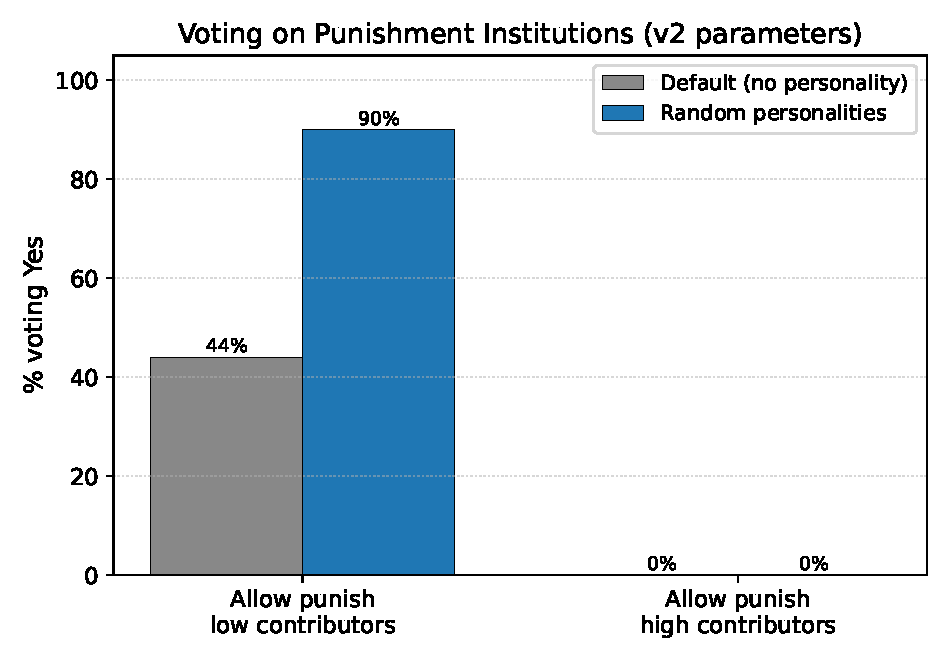
\includegraphics[width=0.75\textwidth]{figures/fig3_voting.pdf}
\caption{Voting on punishment institutions. Both conditions show $0\%$ support for allowing punishment of high contributors, matching the original paper's headline institutional finding. On the punish-low vote, default agents and random-personality agents disagree: default agents vote $44\%$ in favour (below majority), random agents vote $90\%$. See Discussion for why this direction reverses relative to our prior scaled-up replication.}
\label{fig:voting}
\end{figure}

\textbf{Fifth, costly punishment is modest and similar across conditions on all three profiles.} Both conditions spend essentially nothing on the all-cooperate profile ($0.36$ vs $0.30$, $p=0.87$). Both spend a bit on the mixed profile (about $1.4$--$1.7$, $p=0.36$). The only profile where the conditions differ weakly is the one-free-rider scenario ($1.52$ vs $1.96$, $p=0.02$), with random personalities punishing slightly more. None of the punishment-spending results survive Bonferroni correction at $\alpha=0.005$ except for tests where default sits at the exact Nash corner; the punishment-side story in this parameterisation is ``both conditions are similarly mild and both correctly target free-riders when they punish at all.''

\begin{figure}[H]
\centering

\includegraphics[width=0.85\textwidth]{figures/fig4_punishment_by_profile.pdf}
\caption{Mean costly punishment spending by group profile and condition. Both conditions spend essentially nothing on the all-cooperate profile, and spend the most on the free-rider profile. The two conditions track each other closely across profiles.}
\label{fig:punishment}
\end{figure}

\subsection{Within-Subject Regime Effects}

For each condition we ran a Friedman test on the four regime contributions, testing whether the same agent contributes differently across the no-punishment, punish-low-only, punish-high-only, and unrestricted regimes (Table~\ref{tab:friedman}).

\begin{table}[H]
\centering
\caption{Friedman Test of Regime Effects (Within-Subject)}
\label{tab:friedman}
\begin{tabular}{lccc}
\toprule
Condition & $\chi^2$ & $p$ & $N$ \\
\midrule
Default & $110.54$ & $<.001$ & $50$ \\
Random personalities & $126.60$ & $<.001$ & $50$ \\
\bottomrule
\end{tabular}
\end{table}

Both conditions show very strong within-subject regime effects. This is the test the original paper used (as a Wilcoxon signed-rank, its two-condition sibling) to establish that the same subject contributes differently under different punishment rules. Our agents do the same thing: within-subject, regime matters. Default agents move from $0$ in punish-high-only to $7$ in punish-low-only; random agents move from $2.42$ to $8.18$ on the same two regimes. Both shifts are large and the Friedman statistic picks both of them up.

\subsection{Multiple-Comparison Correction}

We ran ten between-condition tests. The Bonferroni-corrected threshold is $\alpha=0.05/10=0.005$. All results in Table~\ref{tab:results} marked with $p<.001$ survive correction. The borderline numeric result (unrestricted contribution, $p=0.047$) and the free-rider punishment result ($p=0.019$) do not survive correction; we report them as suggestive but not confirmed.

As in our prior paper, correction does not change the qualitative story: the main effects (baseline contribution, punish-high contribution, voting on low-punishment) are all orders of magnitude below any correction threshold, and the non-significant or borderline results are non-significant or borderline no matter where you set the bar.

%----------------------------------------------------------------------
\section{Discussion}
%----------------------------------------------------------------------

\subsection{Parameter Matching Flips the Voting Direction}

The most interesting---and least comfortable---result in this replication is the voting flip. Our prior paper, at scaled-up parameters (group $5$, endowment $20$, ratio $1{:}3$), found that default agents voted $94\%$ in favour of allowing punishment of low contributors, and that random-personality agents voted $80\%$ (a non-significant reduction). At original parameters (group $4$, endowment $10$, ratio $1{:}4$), default agents vote $44\%$ in favour---below majority---and random-personality agents vote $90\%$. The direction of the default-to-random effect has flipped.

We think the cleanest reading of this is that the default agent's institutional preference at smaller endowment and cheaper-to-punisher ratio is much more Nash-like than it was at the scaled-up parameters. With an endowment of $10$ and a baseline contribution of $0.76$, the default agent is essentially contributing nothing---so from its own perspective, a punishment institution that targets below-average contributors is one that would target \emph{itself}. That makes a strategic self-interest argument for voting No on the institution, which the majority of default agents in fact do ($28/50$). In the scaled-up parameterisation, default agents contributed more at baseline (about $1.0$ out of $20$, which is a lower fraction but in raw numbers still above zero), and the punishment threshold was scaled differently; the institution was less directly threatening to the agent's own behavior, and the vote swung the other way.

Random-personality agents don't have this problem: they contribute $5.3$ out of $10$, comfortably above-average, and so the punish-low institution doesn't target them. They vote $90\%$ in favour of it. That's the direction the original paper's human subjects moved in after repeated play: toward supporting the institution that targets the free-riders, because the median voter isn't a free-rider.

This is a reasonable and, in some ways, \emph{more} consistent result with the original paper than our prior scaled-up numbers were. The original paper's subjects gradually converged on supporting low-punishment institutions over thirty rounds of play. Our random-personality agents get there in one shot at original parameters. The default agents, playing essentially Nash, don't---which is also arguably correct, because a Nash-playing agent is exactly the kind of agent that an anti-free-rider institution is designed to deter, and they have every strategic reason to vote it down.

The main caveat is that we now have two replications with opposite-signed default-to-random voting effects at different parameterisations, and we haven't yet done the parameterisation-only control that would isolate which specific change (group size, endowment, cost ratio, or their interaction) is responsible. A short future run that varies one parameter at a time would be the right way to close this.

\subsection{Chat Mode, Memory, and Regime Response}

The Friedman tests are the cleanest evidence that chat-mode persistent memory is not hurting performance. Both conditions show highly significant within-subject regime effects, meaning that when the same agent is asked about different punishment regimes, its contribution shifts appropriately. This is the within-subject signal that the stateless mode could also produce in principle (each regime is a separate LLM call in either mode) but in chat mode you get the signal \emph{and} the context: the agent sees its own previous regime answers when reasoning about the next one.

The strongest within-subject shift in either condition is from punish-high-only to punish-low-only. Default: $0.00 \to 7.00$. Random: $2.42 \to 8.18$. Both are large; both happen within the same conversation thread in chat mode. The chat-mode agent does not appear to be stuck in a single fixed strategy---it responds to regime information about as strongly as the prior stateless-mode agent did, and arguably a bit more coherently, because its prior regime answers are visible to it as part of its own history rather than being invisible context from a fresh call.

\subsection{The Dropout Resolved}

The form-completion failure we diagnosed in our prior paper ($43/50$ failed the costly-punishment page in the hyper-cooperative condition at $16{,}000$ tokens) does not occur in either of the conditions reported here at $128{,}000$ tokens. This is exactly the testable prediction our prior paper laid out: raise the token budget, and the dropout should disappear if the mechanism is reasoning-token exhaustion rather than behavioral refusal. $0/50$ failures in each condition confirms the prediction.

This does mean we have not yet re-run the hyper-cooperative condition at the new budget. That is the natural next extension. If the Discussion section of our prior paper was right about the mechanism, the hyper-cooperative condition at $128{,}000$ tokens should complete at $50/50$ and produce full-strength prosocial behavior in the punishment fields. We defer that run to future work but note that we have the infrastructure to do it cheaply.

\subsection{Limitations}

\textbf{Single-shot.} As in our prior paper, agents do not play thirty rounds; they see the four parts in a single oTree session. Conditional cooperation, learning dynamics, and norm-formation effects are not captured.

\textbf{Two conditions only.} We ran default and random personalities, not hyper-cooperative or skewed-disagreeable. The full three-condition gradient of our prior paper is not reproduced here.

\textbf{Model specificity.} Results are specific to \texttt{step-3.5-flash}. A non-reasoning model might show different absolute numbers, though the qualitative pattern (personality shifts baseline contribution up; regime differences are large within-subject; punish-high voting is zero) has held across the models we've tested so far.

\textbf{Ordered-probit regression not applied.} The original paper used ordered-probit regression as its main analytical tool for individual punishment decisions. We've added Friedman and Cohen's $d$ to our statistical chain in this paper, which closes part of the gap with the original methodology, but we have not yet applied regression analyses to individual trait-behavior relationships.

%----------------------------------------------------------------------
\section{Conclusion}
%----------------------------------------------------------------------

We re-replicated \citet{ertan2009who} at the original paper's parameters (groups of $4$, endowment of $10$, punishment cost ratio $1{:}4$) with chat-mode LLM agents that maintain persistent memory across every page of the experiment. Two conditions---default and random Big Five personalities---each produce $50/50$ clean completion, and together they replicate the single most robust finding from the original paper ($0\%$ of agents vote to allow punishment of high contributors, in both conditions) while differing sharply on almost every other dimension we measured.

Three conclusions fall out. First, the original paper's headline institutional result is robust to both parameter changes and personality induction in single-shot LLM agents: no one votes to punish cooperators, period. Second, the baseline contribution is extremely sensitive to whether an agent is given a personality prompt; the same pipeline and same parameters produce contributions of $0.76$ by default and $5.30$ with personality, a seven-fold difference with a Cohen's $d$ of $-2.25$. Third, the dropout effect from our prior paper was a measurement artifact, not a behavioral refusal, and is completely eliminated by raising the reasoning-token budget---exactly as the prior paper predicted.

The most important direction we did not pursue in this paper, and which we view as the single largest gap in the series, remains multi-round design. Porting chat-mode agents to a repeated public-goods game with persistent history across rounds is the natural next step. Chat-mode memory makes that step architecturally straightforward; the only work required is a multi-round oTree app that feeds round-by-round results into the conversation. Running this at original parameters, with the same two-condition contrast, would directly address the learning-dynamics question that the single-shot design cannot.

%----------------------------------------------------------------------
\bibliographystyle{apalike}
\bibliography{refs}

\end{document}
